% Name: Phase-locked loop
% Description: A phase detector, a loop filter, and a voltage-controlled oscillator, with a divide-by-N counter that makes the output N times the reference frequency.
% Tags: PLL, phase-locked loop, frequency synthesis, electronics

\usetikzlibrary{arrows.meta, positioning}

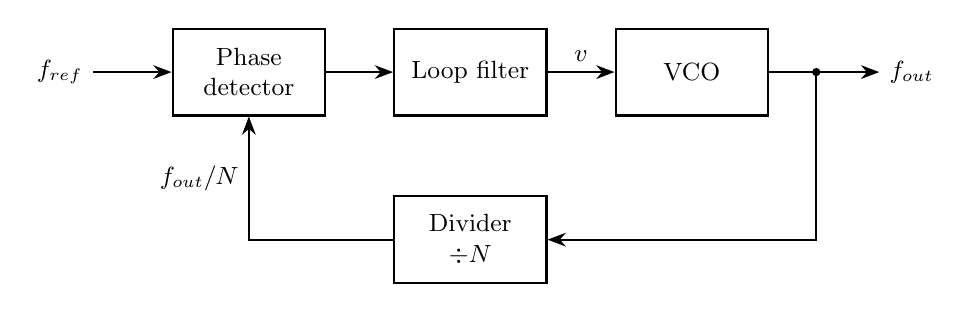
\begin{tikzpicture}[
  node distance=10mm and 8.5mm,
  every node/.style={font=\small},
  block/.style={draw, thick, minimum height=11mm, text width=17mm, align=center},
  arrow/.style={-{Stealth}, thick},
]
  \node[block] (pd) {Phase detector};
  \node[block, right=of pd] (lf) {Loop filter};
  \node[block, right=of lf] (vco) {VCO};
  \node[block, below=of lf] (div) {Divider\\ $\div N$};

  \draw[arrow] ([xshift=-10mm]pd.west) node[left] {$f_\text{ref}$} -- (pd);
  \draw[arrow] (pd) -- (lf);
  \draw[arrow] (lf) -- node[above] {$v$} (vco);
  \draw[arrow] (vco.east) -- ++(14mm,0) node[right] {$f_\text{out}$};
  \draw[arrow] ([xshift=6mm]vco.east) |- (div);
  \draw[arrow] (div) -| node[pos=0.75, left] {$f_\text{out} / N$} (pd);
  \fill ([xshift=6mm]vco.east) circle (1.5pt);
\end{tikzpicture}
